% !TEX root = ../../main.tex

\chapter{Cost Estimation}

\label{chapter:cost-estimation}
In this chapter, we share the results of our experiments and explain how we used these results to build four different cost models. The \hyperref[sec:5-motivation]{first section} shows the results of the experiments, motivating why a cost model is necessary. In \autoref{sec:5-cost-models}, we talk about how we used these results to create the cost models. Each model is made for a specific purpose and offers different ways to solve the problem. This chapter aims to give a clear picture of how we ran the experiments and built the cost models from the results.

\section{Motivation}
\label{sec:5-motivation}
\todo{Simple visualisation to show why cost estimation is needed, and obvious correlations between dependent/independent vars.}
To show the major impact our chosen independent variables have on the trade-off between Materialization and Factorization we first the performance ratio against a range of independent variables. We group the Data and Model characteristics as they both influence the actual computations being executed, whereas the hardware characteristics only influence how these computations are carried out on the hardware.

\subsection{Data \& Model Characteristics}


\subsection{Hardware Characteristics}

\begin{figure}[ht]
    \centering
    \includegraphics[draft, width=0.5\linewidth]{example-image}
    \caption{\todo{Performance ratio against CPU parallelism.}}
    \label{fig:5-cpu-parallelism}
\end{figure}


\begin{figure}[ht]
    \centering
    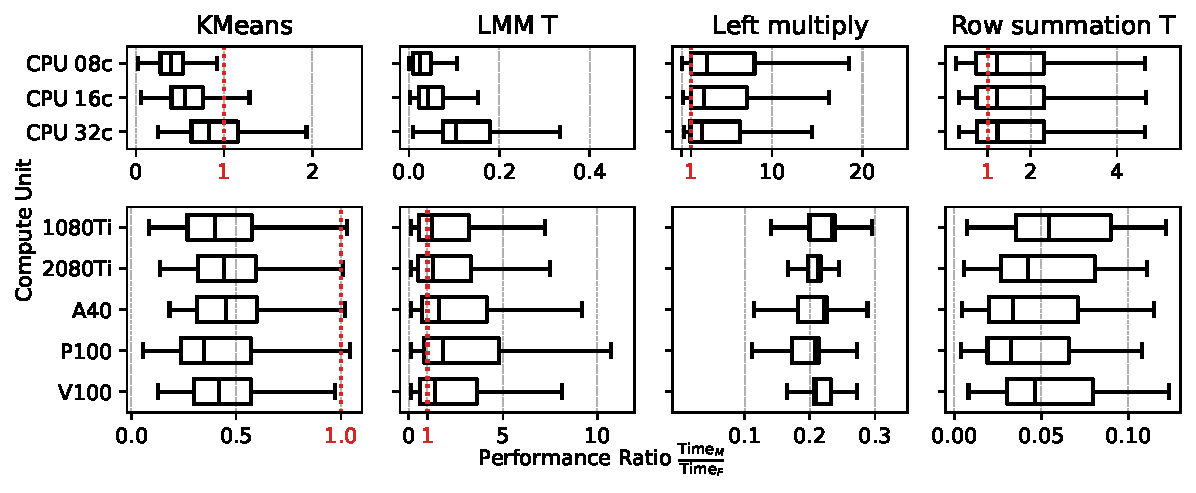
\includegraphics[width=\linewidth]{chapters/05_cost_estimation/figures/motivation_speedup_per_operator_per_gpu.pdf}
    \caption{Performance ratio is shown to dependent on hardware.}
    \label{fig:5-gpu-characteristics}
\end{figure}


\todo{Thus, all factors are very important, and we need complex models to estimate.}

\section{Cost Models}
\label{sec:5-cost-models}
\todo{Detail the full process going from data to Cost model, what features where used, and what is the inner architecture?\\Show each of the factors is significant. Data, Hardware, Model parameters}

\subsection{Feature Engineering}
\label{sec:5-feature-engineering}
\todo{Data Preprocessing steps}


\subsection{Analytical}

\subsection{Statistical}

\subsection{Deep Learning}

\subsection{Hybrid}

\subsection{Meta-results}
\todo{Inference speed, training time.}
